\documentclass[11pt]{article}
\usepackage[ngerman]{babel}
\usepackage{tocloft}
\usepackage{titlesec}
\usepackage{etoolbox}
\usepackage{setspace}
\usepackage{graphicx}
\usepackage{enumitem}
\usepackage{tcolorbox}
\usepackage[skip=0.5em]{caption}
\usepackage[left=2cm, right=2cm, top=2cm, bottom=2cm]{geometry}

\renewcommand*\contentsname{Inhaltsverzeichnis} %defines the name of the toc
\renewcommand*\thesection{2.\arabic{section}} %defines a custom numbering for sections

% sets new length variable, only used for custom environment
\newlength{\subsectionindent}
\setlength{\subsectionindent}{4.2em}
\newlength{\reflexionindent}
\setlength{\reflexionindent}{2.2em}

%defines an environment that applies a custom indent to text inside
\newenvironment{subindent}[1][\subsectionindent]
{%
  \begingroup
  \setlength{\leftskip}{#1}%
  \setlength{\parindent}{0pt}%
}
{%
  \par\endgroup
}

%defines an environment that applies a custom indent to text inside
\newenvironment{refindent}[1][\reflexionindent]
{%
  \begingroup
  \setlength{\leftskip}{#1}%
  \setlength{\parindent}{0pt}%
}
{%
  \par\endgroup
}

%TODO
%general formatting of line seperation and font size
%formatting in general (per chapter)
%colors of tcolorboxes

\begin{document}

% applies a custom font and layout to sections
\titleformat{\section}
  {\normalfont\Large\bfseries}
  {\thesection}{0.5em}{}
\titlespacing*{\section}{0em}{*3}{*1}

% applies a custom font and layout to subsections
\titleformat{\subsection}
  {\normalfont\large\bfseries} % font
  {\thesubsection}{0.5em}{} % section number and space between num and title
\titlespacing*{\subsection}{1em}{*2}{*0.5} % spacing around titles

% forces a fixed indent for EVERYTHING (applies to formatting of boxes and img)
% \makeatletter
% \pretocmd{\subsection}{\setlength{\leftskip}{4.2em}}{}{}
% \pretocmd{\section}{\setlength{\leftskip}{0pt}}{}{}
% \makeatother

\begin{titlepage}
    \begin{center}
        \vspace*{1cm}
        \LARGE
        Lernfeld 2 Portfolio

        \vspace{0.5cm}
        \Huge
        \textbf{Arbeitsplätze nach Kundenwunsch ausstatten}

        \vspace{1.5cm}
        \large
        %\textbf{Christopher Vitz}

        \vspace*{\fill}
        Technisch-Gewerbliches Berufsbildungszentrum Saarbrücken \\
        \today
    \end{center}  
\end{titlepage}

{
\fontsize{12pt}{12.5pt}\selectfont
\cftsetindents{section}{0em}{2.5em}
\cftsetindents{subsection}{1em}{3em}
%toc in need of formatting (line spacing, font size)
\tableofcontents
}

\newpage
\section{Eine Einführung in die IT für Arbeitsplätze geben}
\subsection{Eine Einführung in Grundfunktionen des Computers geben}
    \vspace{0.5em}
    \begin{tcolorbox}[width=9cm, center, title=EVA-Grundprinzip der Datenverarbeitung, coltitle=white, colframe=orange, colback=white!60!orange]
        \begin{itemize}
            \item[E =] Eingabe
            \item[V =] Verarbeitung
            \item[A =] Ausgabe
        \end{itemize}
    \end{tcolorbox}
    \vspace{-0.5em}
    \begin{figure}[h]
        \centering
        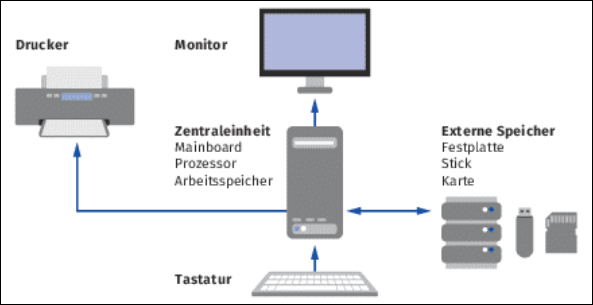
\includegraphics[width=0.7\textwidth]{./images/2.1.1_konfiguration.png}
        \caption{EVA-Prinzip Beispiel}\label{fig:EVA-Prinzip}
    \end{figure}
    \vspace{-0.5em}
    \begin{tcolorbox}[width=13cm, center, title=Konfiguration, coltitle=white, colframe=white!20!blue, colback=white!80!blue]
        Bezeichnung für abgestimmte Zusammenstellung von Hardware und Software auf Nutzungszweck des Kunden.
    \end{tcolorbox}
    \vspace{0.25em}
\subsection{Bedeutende Entwicklungsschritte in der Computertechnik}
    \vspace{0.5em}
    \begin{itemize}[leftmargin=3cm]
        \item[1980er:] IBM, 8Bit Prozessor, 64KB RAM
        \item[1990er:] Open Source, Internet, Google
        \item[2000er:] Open Office, Facebook
        \item[2020er:] KI, 64Bit Prozessor, 64GB+ RAM
        \item[2030er:] Quantencomputer
    \end{itemize}

\newpage
\subsection{Entwicklungstrends präsentieren}
    \vspace{-0.5em}
    \begin{figure}[h]
        \centering
        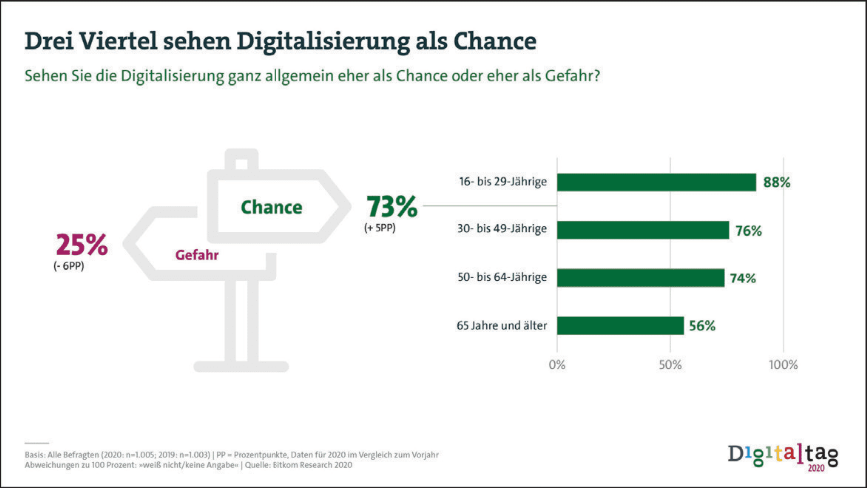
\includegraphics[width=0.7\textwidth]{./images/2.1.3_entwicklungstrend-digitalisierung.png}
        \caption{Entwicklungstrend zur Digitalisierung}\label{fig:Entwicklungstrend_Digitalisierung}
    \end{figure}
    \vspace{-0.5em}
\subsection{Komponentenhersteller und Systemarchitekturen präsentieren}
    \begin{subindent}
        Wichtige Hersteller in der heutigen Zeit:
    \end{subindent}
    \vspace{-0.5em}
    \begin{itemize}[leftmargin=2.5cm]
        \item Intel (Prozessor Marktführer)
        \item AMD (Konkurrent zu Intel)
        \item NVIDIA (Größter Grafikkartenentwickler)
        \item ARM (Prozessorarchitektur)
        \item Apple
        \item Microsoft (Betriebssystem Marktführer)
    \end{itemize}
    \vspace{0.5em}
    \begin{tcolorbox}[width=15cm, center, title=Kompatibilität, coltitle=white, colframe=white!20!blue, colback=white!80!blue]
        Bezeichnung für Verträglichkeit von Komponenten zeinander.
        \begin{itemize}[labelsep=1em, align=parleft, leftmargin=*, widest=Abwärtskompabilität, itemsep=0em]
            \item[Aufwärtskompabilität:] Vorgängerversionen funktionieren mit Nachfolgeversionen
            \item[Abwärtskompabilität: ] neuere Komponenten funktionieren mit Vorgängerversionen
        \end{itemize}
    \end{tcolorbox}
\subsection*{Reflexion Kapitel 2.1}
\addcontentsline{toc}{subsection}{Reflexion Kapitel 2.1}
    \begin{refindent}
        Grundlage zur Verbindung der einzelnen Komponenten eines Computers erlernt (EVA-Prinzip, Konfiguration und Kompatibilität).
        Ebenso ein grobes Wissen über die Entwicklung der IT erlangt, mit möglichen zukünftigen Entwicklungen.
        Verschiedene Hersteller kennengelernt, die einen Großteil des Marktes ausmachen.
    \end{refindent}

\newpage
%TODO Formatting
\section{Das Leistungsportfolio im Ausbildungsbetrieb präsentieren}
\subsection{Arbeitsplätze und Arbeitsumgebungen für IT-Systeme beschreiben}
    \begin{subindent}
        IT ist heutzutage sowohl im privaten sowie industriellen Kontext nicht wegzudenken. \\
        Einsatzbereiche der IT\@:
    \end{subindent}
    
    \begin{itemize}[leftmargin=2.5cm, topsep=0.3em, itemsep=0.1em, parsep=0.5em]
        \item Privat
        \item Industrie
        \item Wirtschaft
        \item Verwaltung
    \end{itemize}
    
    \begin{subindent}
        Formen von Arbeitsarten:
    \end{subindent}
    
    \begin{itemize}[leftmargin=2.5cm, topsep=0.3em, itemsep=0.1em, parsep=0.5em]
        \item Telearbeiten: Arbeiten an einem eingerichteten Arbeitsplatz
        \item mobiles Arbeiten: auch Homeoffice, Arbeit nicht an festen Arbeitsplatz gebunden
    \end{itemize}
    
    \begin{subindent}
        Die Arbeitsplätze dieser Arten sind nach Bürokonzepten gestaltet und müssen ergonomische, ökologische und gesundheitliche Anforderungen berücksichtigen. \\
        Formen von Arbeitsumgebungen:
    \end{subindent}
    
    \begin{itemize}[leftmargin=2.5cm, topsep=0.3em, itemsep=0.1em, parsep=0.5em]
        \item Zellenbüros: Ein-/Mehrpersonenbüros entlang eines FLurs
        \item Großraumbüros: Open-Space-Bürolandschaft
        \item Kombibüro: Einzelbüros entlag der Fassade, Pausenraum dazwischen
        \item Non-Territoriales Büro: Büroplätze werden von Mitarbeitern für Arbeitszeit gebucht
    \end{itemize}
    
    \begin{subindent}
        Bei der Gestaltung der Arbeitsplätze muss auf genügend Beleuchtung (min. 500 Lux) sowie eine nicht zu hohe Lärmentwicklung (30-45dB) geachtet werden.
    \end{subindent}

\subsection{Marktgängige IT-Systeme vorstellen}
    \begin{tcolorbox}[width=15cm, center, title=Konfiguration, coltitle=white, colframe=orange, colback=white!60!orange]
        Bezeichnung für die Zusammenstellung, Einstellung und Abstimmung von Komponenten/Geräten/Programmen in Bezug auf Anwendung. \\
        Unterscheidung vom Istzustand (Ist-Konfiguration) als aktuellem Stand und Sollzustand (Soll-Konfiguration) als Zielzustand.
    \end{tcolorbox}
    %TODO evtl die verschiedenen bauformen adden
    \vspace{-1em}
    
    \begin{figure}[h]
        \centering
        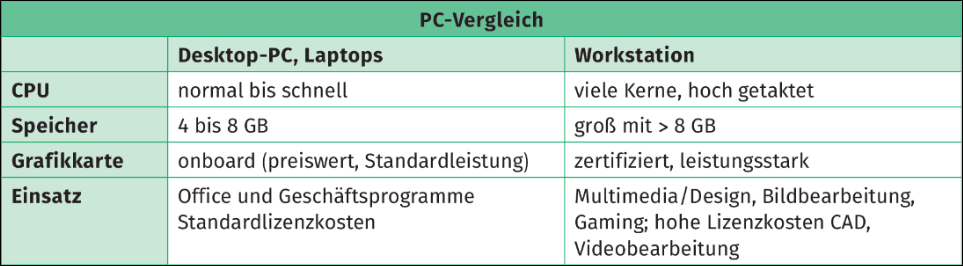
\includegraphics[width=0.7\textwidth]{./images/2.2.2_pc-vergleich.png}
        \caption{Unterscheidung der Leistungsfähigkeit}\label{fig:Leistungsfähigkeit_Unterscheidung}
    \end{figure}
    
    \begin{subindent}
        IT-Hardware kann auf verschiedene Kriterien und Spezifikationen geprüft werden. \\
        Dabei sind die folgenden von besonderer Bedeutung:
    \end{subindent}
    
    \begin{itemize}[leftmargin=2.5cm, topsep=0.3em, itemsep=0.1em, parsep=0.5em]
        \item Quantitative Größen (messbare, objektive Größen)
        \item Qualitative Größen (schwer messbare, subjektive Größen)
        \item Vergleiche (Stress-/Benchmarktests, etc.)
    \end{itemize}
    
    \begin{subindent}
        Desweiteren können zusätzliche Recherchen durchgeführt werden, etwa über das Internet (Fachportale, Blogs, etc.) oder Hardware-Tests und Diagnosetools.
    
    \end{subindent}

\subsection{Das Leistungsportfolio im IT-Bereich präsentieren}
    \begin{subindent}
        Das Leistungsportfolio eines Unternehmens beschreibt die Dientsleistungen und Tätigkeiten eines Betriebs. \\
        Bei Unternehmen mit interner IT, ist die IT-Abteilung der Dienstleister der Mitarbeiter und Abteilungen. Die Mitarbeiter sind demnach interne Kunden.
    \end{subindent}

\subsection*{Reflexion Kapitel 2.2}
\addcontentsline{toc}{subsection}{Reflexion Kapitel 2.2}
    %TODO REFLEXION
    \begin{refindent}
        TODO
    \end{refindent}

\newpage
\section{Auswahlkriterien zu IT-Produkten allgemein unterscheiden}
\subsection{Qualität und Leistungsfähigkeit von IT-Systemen und IT-Services beschreiben}
    \begin{subindent}
        Qualitätsniveau und Qualitätsmanagement werden in der modernen IT immer wichtiger.
        Daher erhöht sich der Anspruch an diese Aspekte innerhalb von Unternehmen stetig. Diese Ansprüche umfassen die in der folgenden Begriffserklärung gelisteten Punkte.
    \end{subindent}

    \begin{tcolorbox}[width=13cm, center, title=Qualitätsbegriff, coltitle=white, colframe=white!20!blue, colback=white!80!blue]
        \begin{enumerate}[itemsep=0.01em, parsep=0.3em]
            \item Beschaffenheit, Merkmal, Eigenschaft, Zustand
            \item Güte aller Eigenschaften eines Objektes, Systems oder Prozesses
            \item Zweckangemessenheit eines Produktes (Produktqualität), einer Dienstleistung (Servicequalität) oder eines Prozesses (Prozessqualität)
        \end{enumerate}
    \end{tcolorbox}

    \begin{subindent}
        Weitere Mängelarten, Mängel und nicht erfüllte Anforderungen, die im Bundesgesetzbuch festgehalten sind:
    \end{subindent}

    \begin{itemize}[leftmargin=2.5cm, topsep=0.3em, itemsep=0.1em, parsep=0.5em]
        \item Sach- und Rechstmangel (§433-435 BGB)
        \item Mangelausschluss (§434, 442 BGB)
        \item Leistungsausschluss (§275 BGB)
    \end{itemize}

    \begin{subindent}
        Bei digitalen Produkten gelten für Unternehmen gegenüber Verbrauchern zusätzliche Regelungen (§327 BGB). \\
        Standards, Normen und Marken:
    \end{subindent}

    \begin{tcolorbox}[width=11cm, center, title=Normen, coltitle=white, colframe=orange, colback=white!60!orange]
        Technische Vorgaben die von Organisationen festgelegt werden. Werden in z.B. Verträgen oder Gesetzen genannt und erhalten dadurch Verbindlichkeit.
        In Gesetzen und Verordnungen ersetzen sie rechtliche Detailregelungen.
    \end{tcolorbox}

    \begin{tcolorbox}[width=10cm, center, title=Abkürzungen, coltitle=white, colframe=white!20!blue, colback=white!80!blue]
        \begin{itemize}[itemsep=0.01em, parsep=0.3em]
            \item[DIN -] Deutsches Institut für Normung
            \item[ISO -] Internationale Organisation für Normung
            \item[IEC -] Internationale Elektrotechnische Normung
            \item[EN -] Normen Europäischer Komitees 
        \end{itemize}
    \end{tcolorbox}

    \begin{subindent}
        \begin{itemize}[leftmargin=2.5cm, topsep=0.3em, itemsep=0.1em, parsep=0.5em]
            \item \textbf{Zertifizierungen:} \\ Prüfdokumente, ausgestellt von anerkannten Zertifizierungsstellen
            \item \textbf{Formfaktoren:} \\ Konstruktionsvorgaben für Größen, Formen und Anschlüsse für Hardware im Markte
            \item \textbf{Marken:} \\ Schutzzeichen, die Unternehmen beim Patent- und Markenamt erlangen können   
        \end{itemize}
    \end{subindent}

    \begin{figure}[ht]
        \centering
        \includegraphics[width=0.7\textwidth]{./images/2.3.1_qualitätskriterien.png}
        \caption{Qualitätskriterien}\label{fig:Qualitätskriterien}
    \end{figure}

\newpage
\subsection{Umweltschutz und Green-IT als wichtige IT-Ziele darstellen}
    %TODO change tcolorboxes to green (cus green it)
    \begin{figure}[ht]
        \centering
        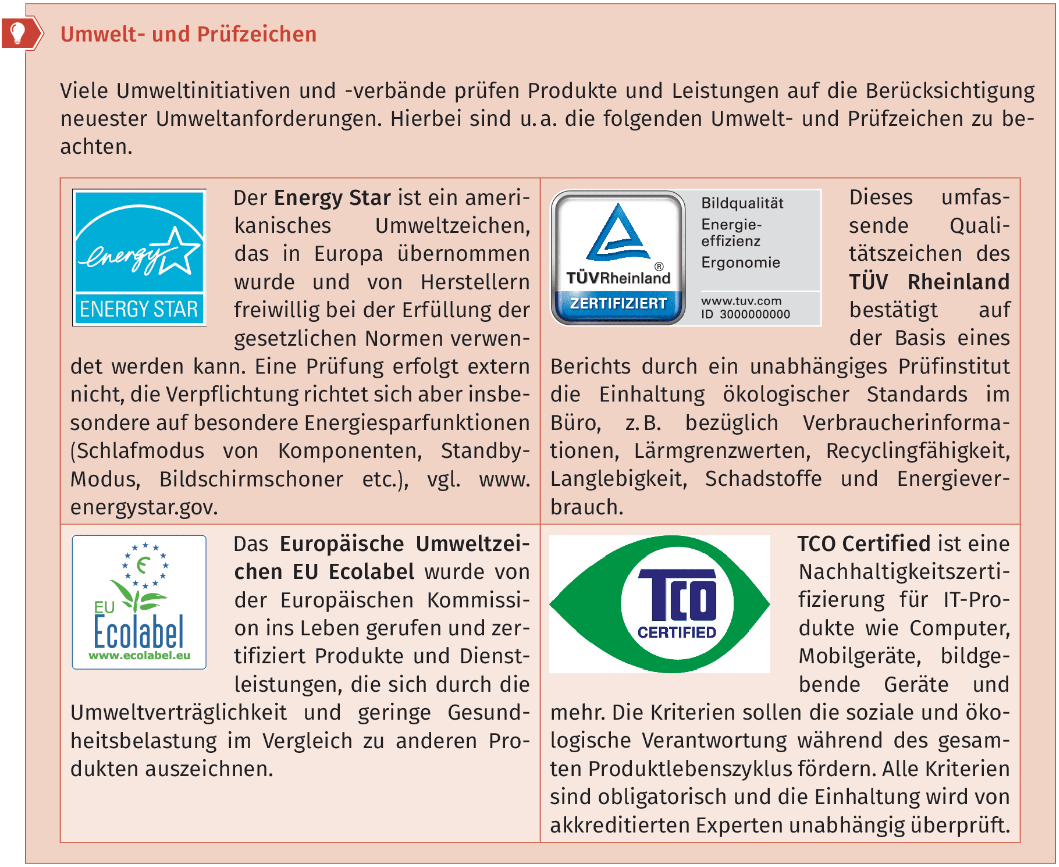
\includegraphics[width=0.7\textwidth]{./images/2.3.2_umweltzeichen.png}
        \caption{Umwelt- und Prüfzeichen}\label{fig:Umweltzeichen}
    \end{figure}

    \begin{tcolorbox}[width=11cm, center, title=Green-IT, coltitle=white, colframe=orange, colback=white!60!orange]
        Unternehmenskultur, IT möglichst umweltschonend zu beschaffen und einzusetzen.\\
        %TODO possible itemize here
        Umfang: Beschaffung, Nutzung, Verwertung und Entsorgung werden als Kreislauf angesehen. Ziel: möglichst wenig Ressourcenverbrauch \\
        Überprüfung: Erstellung von Nachhaltigkeitsrichtlinien, -konzepten, -berichten und -managmentsystemen
    \end{tcolorbox}

    \begin{tcolorbox}[width=14cm, center, title=Maßnahmenkatalog Green-IT, coltitle=white, colframe=orange, colback=white!60!orange]
        \begin{itemize}[itemsep=0.1em, parsep=0.3em]
            \item Bedarfsgerechter Einsatz von Hardware und Software prüfen
            \item Einsparung Energie und Energiekosten durch effiziente IT-Lösungen
            \item Beratung, den Lebenszyklus der Geräte zu verlängern, Kosten zu senken, Refurbished IT einzusetzen
            \item Bedarfsgerechter Betrieb der IT anstelle eines durchlaufenden Betriebs
            \item Energie und Kosten sparen durch Virtualisierung
            \item Einsatz umweltschonender Verbrauchsmaterialien
            \item Software auf Nachhaltigkeit prüfen, eventuell Open-Source-Software vorziehen
            \item Mitarbeiter auffordern, umweltfreundlich zu kommunizieren
        \end{itemize}
    \end{tcolorbox}

\subsection{Wirtschaftlichkeit von IT-Systemen erläutern}
    \begin{subindent}
        In Unternehmen muss wirtschaftlich gearbeitet werden. Hierfür ist bei allen Angeboten eine Wirtschaftslichkeitsbetrachtung durchzuführen, um das beste (nach den folgenden Punkten) zu finden.
    \end{subindent}

    \begin{tcolorbox}[width=11cm, center, title=Wirtschaftlichkeitsbetrachtungskriterien, coltitle=white, colframe=white!20!blue, colback=white!80!blue]
        \begin{itemize}[itemsep=0.01em, parsep=0.3em]
            \item Preisvergleiche
            \item Anschaffungs- und Zusatzkosten
            \item Folgekosten
            \item Restwerte
            \item Sonstige Kriterien (z.B. Lieferantenqualität)
        \end{itemize}
    \end{tcolorbox}

\subsection{IT-Sicherheit von IT-Systemen, Informations- und Datenschutz erläutern}
    \begin{subindent}
        \begin{itemize}[leftmargin=2.5cm, topsep=0.2em, itemsep=0.1em, parsep=0.3em]
            \item \textbf{Datenschutz} \\
                  Schutz privater, personenbezogener Daten eines jeden Menschen
            \item \textbf{Datensicherheit} \\
                  Schutz aller Daten in Unternehmen, unabhängig von Sachbezug oder Personenbezug
            \item \textbf{IT-Sicherheit} \\
                  Allgemeine Bezeichnung für Einsatz von Informationstechnik und den Schutz der damit verbundenen Anforderungen (s.\@ unten)
            \item \textbf{Informationssicherheit} \\
                  Schutz aller Informationen (digital/analog), genauere Eingrenzung durch BSI oder ISO 27001
        \end{itemize}
    \end{subindent}

    \begin{tcolorbox}[width=14cm, center, title=Gemeinsame Anforderungen für Daten und Systeme, coltitle=white, colframe=orange, colback=white!60!orange]
        \begin{itemize}[itemsep=0.1em, parsep=0.3em]
            \item \textbf{Vertraulichkeit:} nur für befugte Personen zugänglich
            \item \textbf{Integrität:} keine Verfälschung, Korrektheit
            \item \textbf{Verfügbarkeit:} Schutz vor Unterbrechungen/Ausfällen
        \end{itemize}
    \end{tcolorbox}
    %TODO S.148-149 Sicherheitsvorfälle und Maßnahmen maybe adden

\subsection*{Reflexion Kapitel 2.3}
\addcontentsline{toc}{subsection}{Reflexion Kapitel 2.3}
    \begin{refindent}
        Qualität und Leistungsfähigkeit werden durch verschieden Normen und Standards garantiert.
        Green-IT ist das Einsetzen von IT nach verschiedenen Nachhaltigkeitsideen/-konzepten.
        (Sehr) kurzer Anriss zu IT-Sicherheit und Maßnahmen dafür.
    \end{refindent}

\newpage
\section{Komponenten eines Arbeitsplatzcomputers unterscheiden}
\subsection{Zentraleinheit, Mainboard und Betriebssystem unterscheiden}
    TODO

\subsection{Hauptplatine, Mainboard und die Komponenten unterscheiden}
    \begin{figure}[ht]
        \centering
        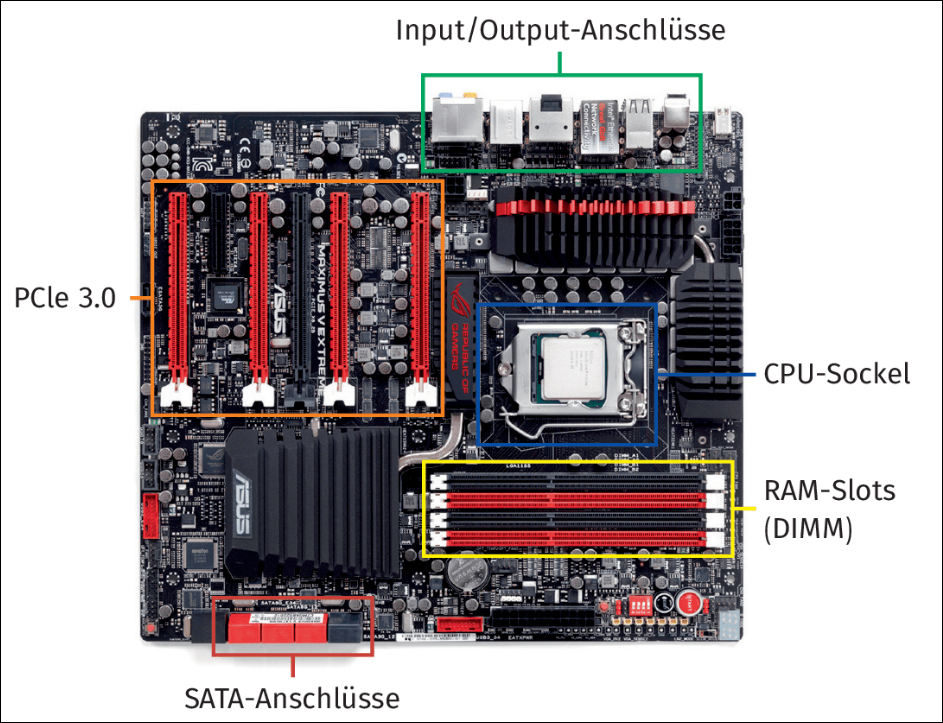
\includegraphics[width=0.7\textwidth]{./images/2.4.2_mainboard.png}
        \caption{Mainboard}\label{fig:Mainboard}
    \end{figure}
    
    \begin{subindent}
        \begin{itemize}[leftmargin=2.5cm, topsep=0.2em, itemsep=0.1em, parsep=0.3em]
            \item \textbf{Mainboard:} \\
                  auch Motherboard oder Systemplatine, Hauptplatine, auf der alle Komponenten angebracht sind
            \item \textbf{BIOS:} \\
                  zuständig für Startvorgang, enthält in \textbf{EPROM} ein Basisbetriebssystem
            \item \textbf{Chipsatz:} \\
                  zuständig für Kommunikation der Komponenten untereinander
            \item \textbf{Sockel:} \\
                  physikalische Verbindung von Mainboard und Prozessor
            \item \textbf{Peripherie-Anschlüsse, (PCIe-)Steckplätze:} \\
                  I/O-Peripherie für externe Hardware (z.B. Maus/Tastatur) \\
                  Steckplätze auf Mainboard für interne Hardware (z.B. RAM, GPU oder SATA/M.2)
            \item \textbf{Netzteil:} \\
                  Stromversorgung aller Komponenten
        \end{itemize}
    \end{subindent}
    
    \begin{figure}[ht]
        \centering
        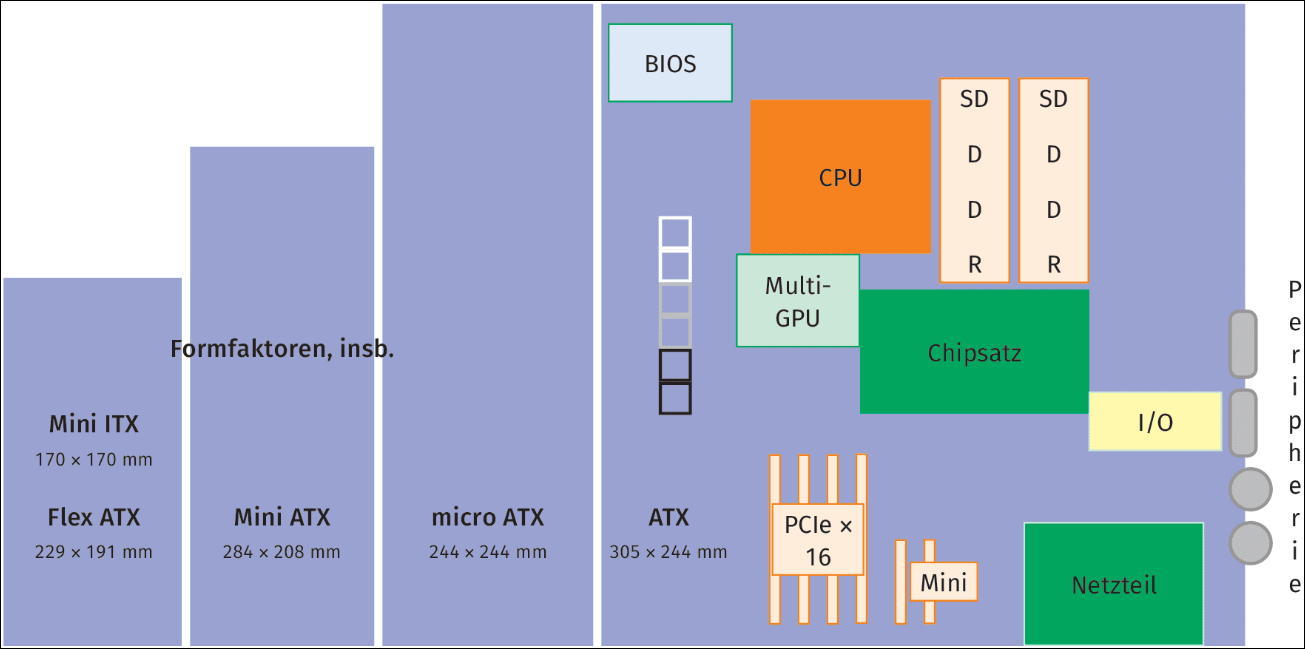
\includegraphics[width=0.7\textwidth]{./images/2.4.2_formfaktoren.png}
        \caption{Formfaktoren}\label{fig:Formfaktoren}
    \end{figure}

\newpage
\subsection{Prozessoren genauer beschreiben}
    TODO

\subsection{Arbeistspeicher (RAM-Speicher) erläutern}
    \begin{subindent}
        RAM-Speicher (Random Access Memory) ist ein flüchtiger Arbeitsspeicher, über den die CPU auf Daten zugreift, wenn mehrere Programme parallel benutzt werden. Da RAM flüchtig ist werden die Daten beim Herunterfahren des PCs gelöscht. \\
        RAM-Formate:
        \begin{itemize}[leftmargin=2.5cm,, itemsep=0.1em, parsep=0.3em]
            \item DIMM\@: Dual In Line Memory Module, wird in Desktops und Servern verwendet
            \item SO-DIMM\@: Small Outline DIMM, wird in Laptops verwendet
        \end{itemize}
        Neben dem Arbeitsspeicher gibt es noch den (im Vergleich zur RAM) schnellen Cache-Speicher. \\
        Cache-Levels:
        \begin{itemize}[leftmargin=2.5cm, itemsep=0.1em, parsep=0.3em]
            \item L1-Cache: Geschwindigkeit ähnlich zu Prozessor, für häufig verwendete Befehle und Daten
            \item L2-Cache: größer und langsamer als L1, aber schneller als RAM
            \item L3-Cache: Datenabgleich Caches und Cores
        \end{itemize}
    \end{subindent}

    \begin{figure}[ht]
        \centering
        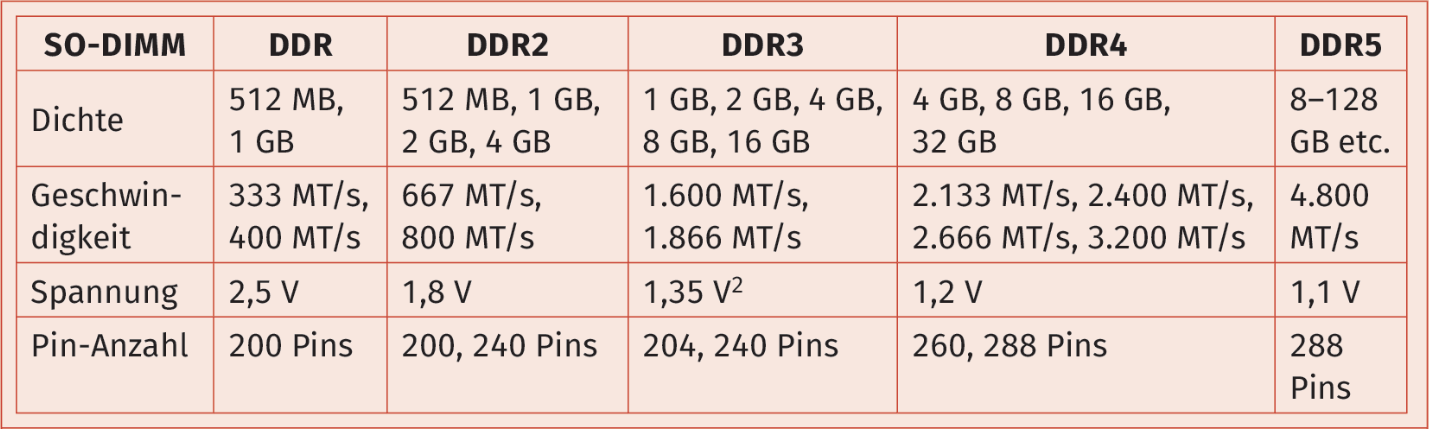
\includegraphics[width=0.7\textwidth]{./images/2.4.4_ramspeeds.png}
        \caption{RAM-Geschwindigkeiten}\label{fig:RAM-Geschwindigkeiten}
    \end{figure}

    \begin{tcolorbox}[width=15cm, center, title=RAM Begriffe, coltitle=white, colframe=orange, colback=white!60!orange]
        \begin{itemize}[itemsep=0.1em, parsep=0.3em]
            \item RAM\@: Random Access Memory
            \item JEDEC\@: \\ Joint Electronic Device Engineering Council \\ Organisation legt Spezifikationen für elektrische und zeitliche Parameter der Speichercontroller und -chips fest
            \item Formfaktoren: \\ UDIMM (Unbuffered DIMM): häufigstes Format in Desktops \\ SO-DIMM\@: kleiner und physikalisch kürzer als UDIMMS
            \item DRAM\@: Dynamic Random Access Memory \\ Jedes Datenbit wird auf seperatem Kondensatoren gespeichert
            \item SDRAM\@: Synchronous Dynamic Random Access Memory \\ getaktetes DRAM, Daten werden synchron zum Speicher-Bus übertragen
            \item DDR-RAM\@: Double Data Rate RAM \\ überträgt Daten doppelt so schnell wie SDRAM\@; neueste Generation ist DDR5 (Gens untereinander nicht kompatibel)
            \item DDR-SDRAM\@: Weiterentwicklung der SDRAM-Technologie
            \item SSD-RAM\@: Solid State RAM \\ flash-based Speicher, SSD-Speicher wird als zusätzliche RAM benutzt, die Daten darauf bleiben beim Herunterfahren erhalten
            \item QLC\@: Quad-Level-Cells \\ neueste Tech der Flash-Speicherarchitektur, speichert vier Datenbits in jeder Datenzelle
            \item FSB\@: Frontsidebus \\ Hauptpfad für Daten im Computer, verbindet CPU, DRAM, GPU und Chipsatz
            \item Latenz\@: Zeit, die Speicher benötigt, um auf Befehl zu reagieren
            \item ECC\@: Error Correcting Code \\ teures `fully buffered, registered ECC RAM', das hilft Speicherfehler zu minimieren oder selbst zu korrigieren 
        \end{itemize}
    \end{tcolorbox}

\subsection{Schnittstellen und Anschlüsse am Mainboard erläutern}
    TODO
\subsection{Netzteile beschreiben und unterscheiden}
    TODO
\subsection{Festplatten unterscheiden und erläutern}
    TODO
\subsection{Tastaturen unterscheiden und präsentieren}
    TODO
\subsection{Monitore vergleichen und präsentieren}
    TODO
\subsection{Leistungsmerkmale für Drucker und Zusatzanforderungen erläutern}
    TODO (aktueller Fortschrittsstand)
\subsection{Scanner beschreiben und für Arbeitsplatz auswählen}
    TODO
\subsection{IT-Zubehör für die Barrierefreiheit und im Aftersales unterscheiden}
    TODO
\subsection{Unternehmenssoftware anbieten und vergleichen}
    TODO
\subsection{Marktgängige IT-Systeme und Lösungen anbieten}
    TODO
\subsection*{Reflexion Kapitel 2.4}
\addcontentsline{toc}{subsection}{Reflexion Kapitel 2.4}
    %TODO REFLEXION
    \begin{refindent}
        TODO
    \end{refindent}

\newpage
\section{Kundenanforderungen im Leisuntgsprozess berücksichtigen und Projektmanagement vorbereiten}
\subsection{Anforderungen zur Kundenzufriedenheit in den Leistungsprozess einbeziehen}
    TODO
\subsection{Marketing- und Verkaufsförderungsmaßnahmen unterstützen}
    TODO
\subsection{Auftragsbearbeitung mit Projektmanagement unterstützen}
    TODO
\subsection*{Reflexion Kapitel 2.5}
\addcontentsline{toc}{subsection}{Reflexion Kapitel 2.5}
    %TODO REFLEXION
    \begin{refindent}
        TODO
    \end{refindent}

\newpage
\section{Bedarfs- und Anforderungsanalysen durchführen}
\subsection{Den Prozess der Anforderungsanalyse erläutern}
    TODO
\subsection{Kundenanforderungen formulieren}
    TODO
\subsection{Hardware- und Systemvorraussetzungen prüfen}
    TODO
\subsection*{Reflexion Kapitel 2.6}
\addcontentsline{toc}{subsection}{Reflexion Kapitel 2.6}
    %TODO REFLEXION
    \begin{refindent}
        TODO
    \end{refindent}

\newpage
\section{Pflichtenhefte erstellen}
\subsection{Anforderungsanalysen zu Desktops und Workstations durchführen}
    TODO
\subsection{Anforderungsanalysen zu Laptops und Tablets durchführen}
    TODO
\subsection{Anforderungsanalysen zu Thin Clients durchführen}
    TODO
\subsection{Desktop as a Service, Miete, Finanzierung und Leasing als Dientsleistungen berücksichtigen}
    TODO
\subsection*{Reflexion Kapitel 2.7}
\addcontentsline{toc}{subsection}{Reflexion Kapitel 2.7}
    %TODO REFLEXION
    \begin{refindent}
        TODO
    \end{refindent}

\newpage
\input{chapters/2_8_angebote-stundensätze.tex}

\newpage
\section{Lieferung, Installation und Übergabe vornehmen}
\subsection{Vorbereitung der Abnahme von Produkten und Leistungen}
    TODO
\subsection{Arbeitssicherheit und Gesundheitsschutz bei der Arbeit gewährleisten}
    TODO
\subsection{Für IT-Sicherheit am Arbeitsplatz eine Risikoanalyse vorbereiten}
    TODO
\subsection{Abfall- und Recyclinggesetze beachten}
    TODO
\subsection{Systemlieferung, -installation und -übergabe als Prozess präsentieren}
    TODO
\subsection*{Reflexion Kapitel 2.9}
\addcontentsline{toc}{subsection}{Reflexion Kapitel 2.9}
    %TODO REFLEXION
    \begin{refindent}
        TODO
    \end{refindent}

\newpage
\section{Kontrolle und Reflexion von Unterricht und betrieblicher Mitarbeit}
    TODO

\end{document}